 \chapter{Introduction}

 \section{Background and Motivation}
 
%In the last decades, mortalities caused by heart diseases 
\textcolor{black}{Heart-related mortality rate has been increasing dramatically due to the} aging of population, chronic cardiovascular diseases and increasing life stress and pace of modern life\cite{mortality}. According \cite{SCDnumber}, %to heart disease and stroke statistics
cardiac diseases are the most common cause of sudden cardiac death (SCD) with 250 000 to 300 000 mortalities in the U.S. every year accounting for 14.7\% of total deaths\cite{SCDnumber}. As World Health Organization reported, 31\% of global deaths are related to cardiovascular diseases (CVDs)\cite{who}. % Therefore, heart disease is called as “Plague of The Times”. In China, there are about 540,000 sudden cardiac deaths every year.In addition, heart diseases tend to attack younger generations, manifested by the increasing proportion of young patients.
These facts fully reflect that heart diseases are threatening the general health of human beings. %Meanwhile since SCD can occur, most likely, without warning and apparent symptoms in advance, the prediction and early recognition of cardiac disease are considered challenging\cite{circulation2010}. 
\textcolor{black}{Since death from CVD can occur in most cases without prior warning and obvious symptoms, it is of a great importance to enable a timely treatment of heart diseases. For this purpose, prevention principles and guidelines which covers age, family history and other potential risk factors causing CVD are deployed in most clinical modeling methods\cite{smith2004principles}. However, these methods require complex manual analysis by trained physicians. Taking this issue into consideration, developing a cost-effective automatic analysis for CVD prevention based on computer is a critical need.}
%Therefore it is of important significance to treat heart diseases timely by early detection and prediction of CVDs. 
More specifically, since most CVDs are accompanied with arrhythmia, accurate and timely recolonization of arrhythmia is a key factor for effective prevention of heart diseases. %effectively and determine definitive therapies for CVDs.

Electrocardiogram (ECG) is the most common way of monitoring hearth functionality, which %recorded for the first time by Waller in 1887, 
contains abundant physiological and pathological information that reflects the heart rhythm and status of various parts of the heart. ECG signal are recorded for the first time by Waller in 1887\cite{besterman1979waller}. %a professor of physiology at Queen Mary Hospital of Royal Society, by using the capillary electro-meter on hearts of dogs and human in 1887.
It records signals generated by electrical activities of heart as a time series. As a noninvasive examination method, it is known to be highly reliable in reflecting functionality of heart. For this reason, ECG has become one of the most conventional technologies (ECG, clinical examination, radiation and ultrasonic inspection) in modern hospitals and clinics, serving as an important reference for doctors' diagnosis of heart diseases\cite{kreger1987electrocardiogram}.


The traditional diagnosis based on ECG analysis are mainly performed by physicians through visual observation and interpretation.%accomplished manually by physicians. According to working experiences and rich knowledge in heart diseases, experts observe and analyze ECG waveforms visually and make accurate diagnosis. 
However, the approach costly and impractical when continuous monitoring \textcolor{black}{of patients is required (e.g. to recognize CVD conditions).}%for CVDs is required. 
There are tremendous ECG records generated everyday, all demand for timely diagnosis and analysis. %Facing with the severe shortage of physicians, automatic 
\textcolor{black}{Due to the limitations in the access to experienced physicians, automated  ECG classification systems have been introduced and became popular soon afterwards} to generate real-time analysis result and provide additional information to physicians. 

Several computer-based automated classification algorithms has been developed by researchers in the last decades \textcolor{black}{to minimize human intervention or to assist physicians with more accurate diagnosis by reducing human mistakes \cite{lagerholm2000clustering, prasad2003classification, autofs, ceylan2009novel, osowski2004support, Hu_et_al,deChazal2006,llamedo2012automatic,bbnn,ince2009generic,Kiranyaz}.} \textcolor{black}{Moreover, with the emerging application of smart health and smart cities, a constant monitoring and analysis of ECG and other physiological signals with direct experts' intervention deems impossible. Therefore,} applying conventional classification algorithms on biomedical signals remains challenging, especially for applications of spontaneous disease detection. 


%0959-4965%
%A typical feature of cardiovascular disease is its spontaneous occurrence. 
\textcolor{black}{A typical feature of cardiovascular disease is the wide range of causing factors and difficulty of recognizing some implicit symptoms before occurrence\cite{wilson1998prediction, whooley2008depressive}. Failing to predict life threatening CVDs} %This unpredictability 
is the principal cause of high mortality for patients with heart disease. 
\textcolor{black}{A timely prediction of hearth abnormalities before their actual occurrences }%An informative anticipation of abnormality 
would enable a therapeutic intervention %ahead of mortal occurrence and thus minimize 
before the condition becomes detrimental, which minimizes the risk of mortality. Nevertheless, the majority of developed conventional ECG classification systems  \textcolor{black}{are only able to detect abnormalities when they occur. To the best of our knowledge, no research work is devoted to the prediction of heart abnormalities ahead of time, which is the main focus of this project\cite{jambukia2015classification, advancewarning}.} %haven't focused on real-time or predicting performance. To address these problems, we propose in this thesis novel non-linear transformation based classification systems with the capacity to predict abnormality.

\textcolor{black}{Another important property of ECG waveforms is their inherent variability among different individuals and due to different physical and environmental conditions including but not limited to gender, age, body-mass index, elevation and air pressure, humidity, temperature, and etc\cite{agesex,intervaria}.}
%Another important property of ECG waveform is its variability caused by distinct physical conditions of different individuals (i.e. gender, age, body-mass index etc.)\cite{agesex,intervaria}. 
Conventional classification algorithms do not easily generalize, when %fall short of generalization when 
applying to different patients' records\cite{llamedo2012automatic}. 
Due to the inter-patient variation in ECG signals and the complexity of cardiac pathological information analysis, most of the existing ECG analysis software only serve as auxiliary devices for physicians. The final results of diagnosis still depend on manual labeling by cardiologists. \textcolor{black}{Recently, several novel patient-specific ECG analysis methods are proposed. Broadly speaking, in these methods systems parameters are adaptable according to individual ECG signal properties\cite{Hu_et_al,deChazal2006,llamedo2012automatic,bbnn,ince2009generic,Kiranyaz}. Some algorithms combine cardiologist manual annotations with automatically generated labels and train personal classifier with updated labels for each individual\cite{Hu_et_al,deChazal2006,llamedo2012automatic}. This design still requires experts' assistance in order to accurately classify ECG signal. Another design in to train a patient-specific classifier using only the patient's ECG signal. Whereas this method fails when a certain type of abnormal signal is not included in the limited personal ECG signal data.}%More importantly, the diagnostic accuracy of the automatic analysis system of the ECG signal still cannot reach the highest diagnostic accuracy of the clinician.


The automatic analysis of ECG signals includes a wide range of techniques. In this work, we focus on overcoming the two drawbacks of existing automatic ECG classification systems, namely the failure in capturing patient-specific variability and the lack of predictive power.%which is patient-specificity and predicting capacity. 
This research aims at improving the inter-patient classification performance and prediction capability of ECG-based diagnosis methods. Our proposed method can revolutionize the current practice of healthcare service by enabling early detection of heart abnormalities, with applications to high-risk people, senior people, and athletes. It also can significantly reduce the mortality rate of SCD. %automatic analysis and recognition of arrhythmia with ECG signals, which has significance in efficient early detection of CVDs and reduce mortality rate of SCD. 

\section{ECG and Arrhythmia}

Electrocardiogram is widely used to monitor the electrical activities of heart and assist diagnosing fatal cardiac diseases. In order to design algorithms specifically for ECG analysis, it is important to develop an insightful perception of the functionality of heart and ECG waveforms.  

\subsection{Characteristics of ECG signal}

A ECG signal reflects the periodical electric signals generated by a heart. Fig.\ref{fig:cardiac_cycle} demonstrates the typical signal waveform for a cardiac cycle (i.e. a heartbeat), which is usually composed of three main waves including P wave, QRS complexes and T wave. These waves corresponds to different physiological activities of the heart. P waves are generated by atrial depolarization which represents the process of pumping blood to ventricles. QRS complexes as the most significant electric activities are caused by the \textit{ventricular} contraction, which is the process of pumping blood to lungs and the rest of the human body. Finally, T waves are the result of \textit{ventricular} repolarization, which is a required recovery process before the following cardiac cycle. Accurate detection and segmentation of each wave is necessary for a profound ECG analysis. The waves are usually represented by their peak locations, also called fiducial peaks. By detecting the most significant peak within QRS complexes (e.g. R peak) automatic algorithms are able to discriminate between two adjacent cardiac cycles. The interval between two R peaks is called RR interval, which is also the inverse of heart rate. Fig.\ref{fig:cardiac_cycle} represents a typical cardiac cycle with the aforementioned intervals.

 \begin{figure}[t]
 	\centering
 	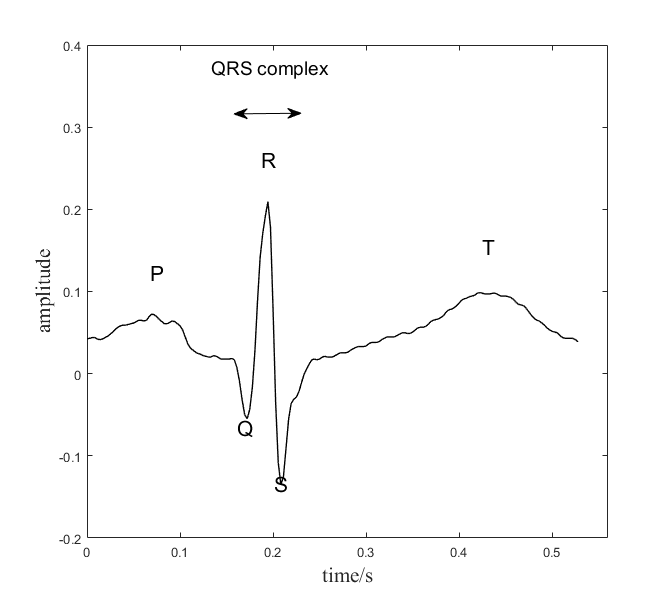
\includegraphics[scale=0.75]{Fig/cardiac_cycle.png}
 	\caption{A typical cardiac cycle in ECG signal with five characteristic waves.}
 	\label{fig:cardiac_cycle}
 \end{figure}

\subsection{MIT-BIH Arrhythmia Database}

Arrhythmia is related to various morbid behaviors of heart. Generally speaking, arrhythmias consist of two main categories: \textit{supraventricular} and \textit{ventricular}. \textit{Ventricular} ectopic beats imply abnormal activities in the ventricles while \textit{supraventricular} ectopic beats are related to the \textit{atria}\cite{houghton2014making}. Both categories contains fatal abnormal beats, which may lead to death\cite{ng2006treating}. Therefore, in order to help researchers standardize the evaluation of works on ECG classifiers, Association for the Advancement of Medical Instrumentation (AAMI) has proposed recommendations for reporting ECG classifier performance\cite{aami}. 
According to these recommendations, MIT-BIH Arrhythmia Database (MITDB) is regarded as a standard database to train and test ECG classifiers in the last two decades. MITDB is a public database which is available on Physionet.com \cite{physionet} since 1997\cite{mitdb}. There are 48 records collected from 47 individuals in this database. Each record contains two channels of ECG raw signals along with annotations for each cardiac cycle. Annotated labels include 16 types, as shown in Table \ref{table:grouping_types}. Among these two channels, \textit{MLII} is more informative and commonly used in automated ECG analysis system, we adopt the signal from this channel as system input\cite{karpagachelvi2010ecg}. Cardiac cycles are determined by the locations of R peaks. %composed of 16 types and R peak locations provided by cardiologists. 
The sampling frequency of MITDB is 360Hz and the signal frequency spans from 0.1 to 100 Hz. 

Following the recommendations by AAMI, the original annotations of MITDB are further grouped into 5 major classes: class N(\textit{normal} and \textit{bundle branch block} beat types) class V(\textit{ventricular} type), class S(\textit{supraventricular} type) and class F(fusion of normal and \textit{Ventricular} types). The class Q which includes unclassified and paced beats are discarded due to the limited number of samples. Table.\ref{table:grouping_types} summarizes the mapping from 16 original types that include cycles of this type. Therefore, only 4 remaining types (N, V, S, F) are typically used.%in annotation to the standard 5 types recommended by AAMI:

\begin{table}[h]
\centering
\caption{Mapping from 16 original types in annotation to the standard 5 types recommended by AAMI}
\label{table:grouping_types}
\begin{tabular}{|c|c|}
\hline
Standard Types by AAMI & Original Types in MITDB Annotation \\ \hline
N                      & NOR, LBBB, RBBB, AE, NE            \\ \hline
V                      & PVC, VE, VF                        \\ \hline
S                      & APC, AP, BAP, NP                   \\ \hline
F                      & VFN                                \\ \hline
Q                      & PACE, FPN, UN                      \\ \hline
\end{tabular}
\end{table}



%For the purpose of training and evaluating classifier, MITDB is split into test (DS2) and training (DS1) set by balancing the four classes according to \cite{autofs}. 

\section{Problem Statement}

ECG signals are investigated broadly by researchers to design automated non-invasive diagnosis methods and real-time monitoring systems\cite{Kiranyaz, chen2018predictive, jchen}. As described in the previous section, a majority of current methods suffer from two main challenges: i) failure to capture inter-patient variability and ii) incapability of early detection and prediction. %To address these problems, we propose in this thesis two novel nonlinear transformation based patient-specific classification systems with the capacity to predict abnormality.

In conventional classification systems, the training dataset is typically composed of records collected from different patients with experts' annotations per heartbeat. In order to unify the records from different patients, most of the conventional classification algorithm \textcolor{black}{mix heartbeat samples from different individual ECG records and cluster the pooled ECG dataset simply based on the annotations of heartbeats.} %concatenate heartbeats from different records and thus result in a pooled ECG dataset. 
Since the classification performance is measured based on the comparison between the predicted labels with the annotate (true) labels for each sample, the classifiers are trained to improve the performance on pooled ECG data. While ECG signals shares similar morphologies, the signals from different patients demonstrate considerable variability as shown in Fig.\ref{fig:interpatient_variability}. Ignoring this difference will lead to inconsistent classification performance between patients. Therefore it's of significant importance to adjust classifier configuration according to patient-specific characteristics.  %A patient-specific classification system refers to systems with cert

 \begin{figure}[thpb]
 	\centering
 	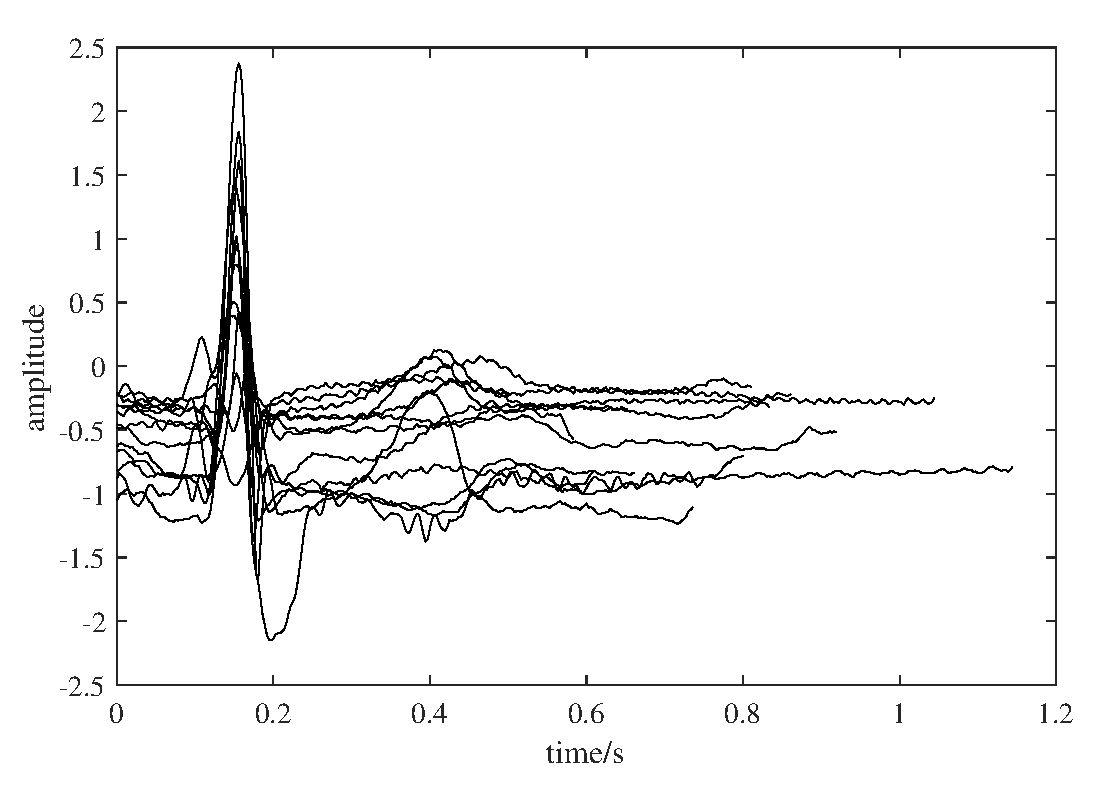
\includegraphics[scale=0.7]{Fig/interpatient_variability.pdf}
 	\caption{ECG signals of normal heartbeat from 15 different records in MIT-BIH reflect the inter-patient variability of ECG signal.}
 	\label{fig:interpatient_variability}
 \end{figure}

In addition to the inter-patient variability, majority of ECG classification algorithms fail to provide a predictive capability, which refers to the power of triggering corresponding alarms before the occurrence of abnormalities. Typically alarms represent significant distortions in the ECG morphology which reflect a severe heart abnormality. The rest of heartbeats considered as \textit{normal} beats. However, an abnormal beat may include mild distortions that can be indicative of a problem, while it is not severe enough to call a \textit{red alarm}. In this work, we represent these minor deviations with \textit{yellow alarm} and use them to predict real abnormalities as \textit{red alarms}, before their actual occurrence.

Fig.\ref{fig:pred_signals} illustrates this concept, where observation of minor deviations from the patient-specific normal trends (\textit{yellow alarms} ) can be indication of upcoming severe abnormalities (\textit{red alarms}). Supporting results are provided in Section \ref{sec:result1} and Section \ref{sec:result_spatial}.%By comparing the morphology of signals which shows salient similarities to abnormal signals precedent to morbid heartbeats with annotated abnormal signal, the potential latent status between abnormal and normal signals is partially demonstrated. If abnormalities in cardiologist annotation are represented by red alarms, thus a system which is able to trigger a corresponding yellow alarm precedent to the abnormality can be considered as capable of predicting abnormalities as shown in Fig.\ref{fig:pred_signals}. 
Therefore, a method to quantify the level of signal similarity to abnormalities should be incorporated into the ECG classification system.

 \begin{figure}[t]
 	\centering
 	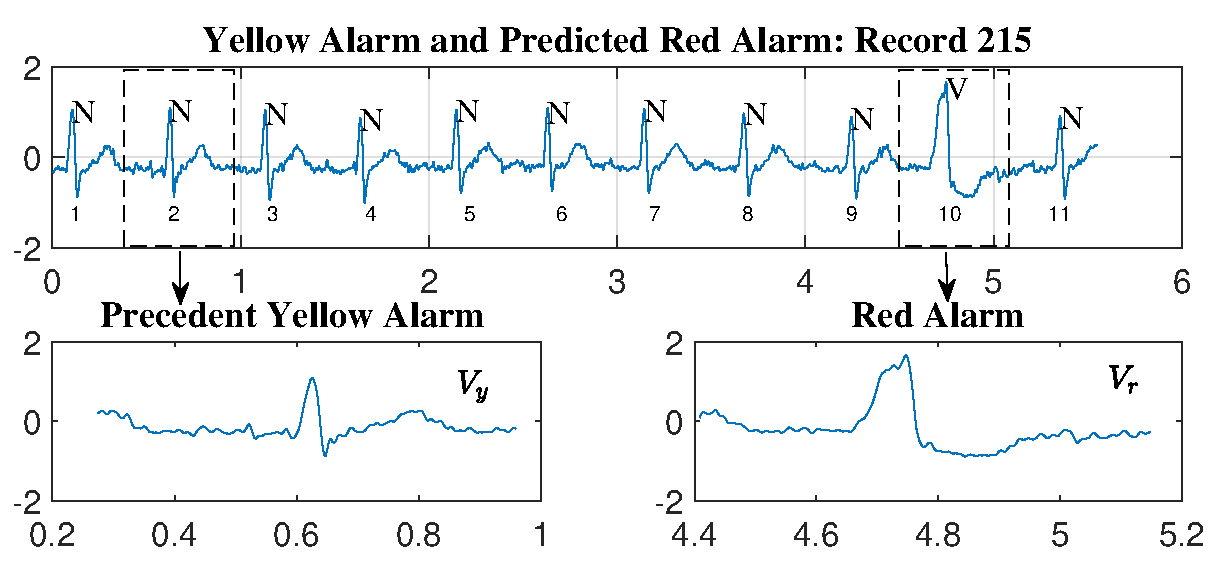
\includegraphics[scale=0.6]{Fig/predicting_record215S_numbered.pdf}
 	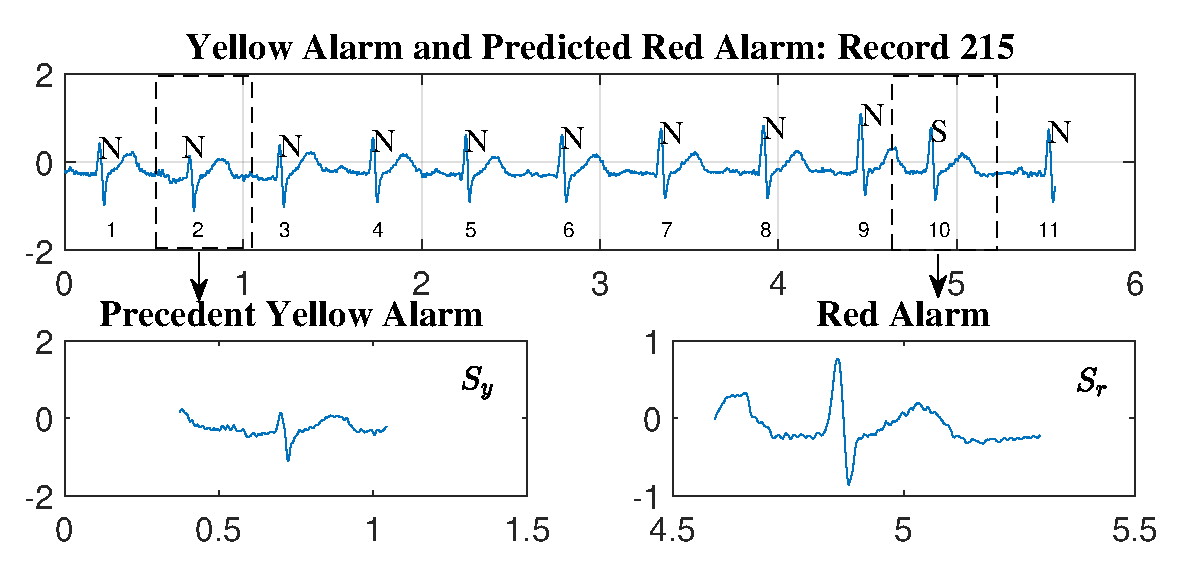
\includegraphics[scale=0.62]{Fig/predicting_record215_numbered.pdf} 
 	\caption{A \textit{yellow alarm} represents a minor abnormality which can be indicator of an upcoming severe abnormality of the same type in terms of a \textit{red alarm}.}
 	\label{fig:pred_signals}
 \end{figure}




\section{Literature Review}
Automatic analysis of ECG signals refers to the entire process spanning from the acquisition of signals to the classification of samples. This process can be divided into five stages: ECG signal acquisition, preprocessing, fiducial peak detection and segmentation, feature extraction and predictive modeling (Fig. \ref{fig:1-1}). Different research works focused on one or multiple stages of the automatic analysis system. Since the main objective of this work is addressing problems in classification algorithms, the literature reviews in this section focuses on studying existing methods proposed for stages before classification, conventional classification algorithms along with patient-specific classification systems. 

 \begin{figure}[thpb]
 	\centering
 	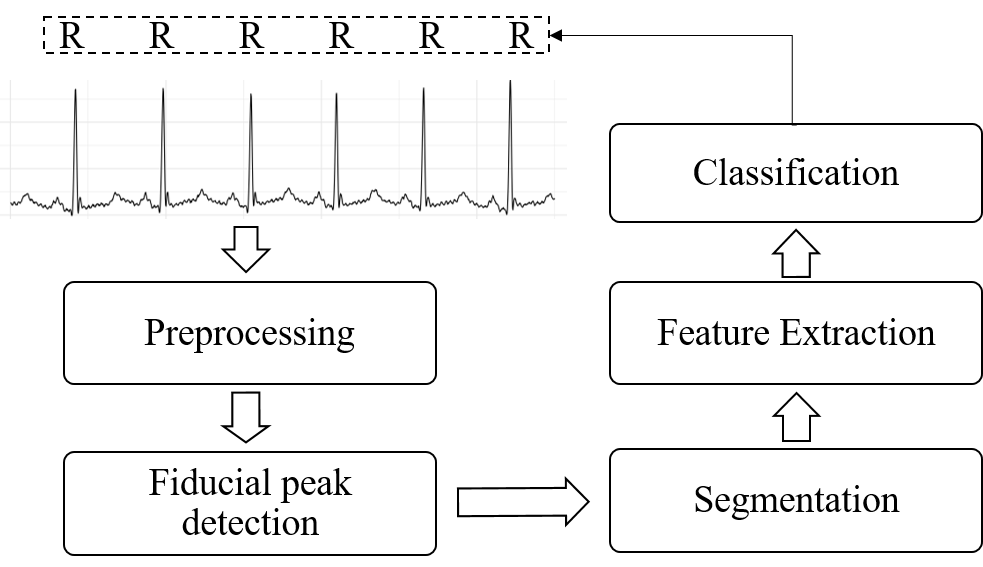
\includegraphics[scale=0.7]{Fig/general_flow.png}  
 	\caption{General structure of ECG analysis system.}
 	\label{fig:1-1}
 \end{figure}


\subsection{ECG Signal Preprocessing}

During data acquisition, the ECG signal may be affected by  different kinds of noise including physiological noise (e.g. myoelectricity noise, breathe interference etc.) and non-physiological noise (e.g. power-frequency interference and electrode impedance interference) \cite{denoise}.These noises often interfere with the informative signal and thus influence the ECG classification results. Therefore, ECG signal preprocessing mainly focuses on the suppression of noise and interference terms in the ECG signal.

The ECG signal is in millivolt (mV) level with a central frequency ranging from 0 to 40 Hz\cite{thakor1984estimation}. %Since ECG signal is comparatively weak with superposition of various noise, 
Due to the relatively low signal to noise ratio in ECG signals, signal preprocessing is a necessary step before classification. Therefore, various methods are proposed to eliminate noise and other artifacts from the ECG signal\cite{lian2004ecg,thakor1984estimation,bai2004adjustable,Sayadi,park1998application, nikolaev2000wavelet, denoise,poungponsri2013adaptive}.%For this purpose, many researches have been conducted targeting different noise component in ECG signal.

Generally speaking, ECG signal preprocessing methods includes finite impulse response (FIR) filtering, adaptive filtering, and modern signal processing filter methods such as wavelet transforms and neural networks\cite{bai2004adjustable,Sayadi,denoise,poungponsri2013adaptive}. YW Bai \textit{et al.} compared different notch filters and concluded that equiripple notch filter outperforms other methods in terms of noise reduction and CPU time\cite{bai2004adjustable}. Lian \textit{et al.} \cite{lian2004ecg} designed a multiplier-free finite impulse response (FIR) filter to surpress biological and environmental noises with a low power consumption. Sayadi \textit{et al.} proposed a modified extended Kalman filter with estimated hidden state variables to perform denoising and compression at simultaneously\cite{Sayadi}. Park \textit{et al.} designed a wavelet-based adaptive filter to reduce S-T segment distortion due to the baseline drift and compared its performance with general adaptive filters\cite{park1998application}. A general conclusion is that the performance of wavelet adaptive filtering is usually higher than generic adaptive filters. In \cite{nikolaev2000wavelet}, the authors combined wavelet decomposition with Wiener filtering to filter out the noise by thresholding, which is proved to outperform other thresholding denoising methods. Regarding various wavelet basis functions, Singh \textit{et al.} studied an optimal selection of basis functions for ECG signal denoising\cite{denoise}. By comparing the classification root mean square error using the same classifier and different denoising methods, they concluded that Daubechies filter of order 8 is the best choice for ECG classification system.


\subsection{Fiducial Peak Detection and Segmentation}\label{sec:fiducial_peaks}

Fiducial Peak Detection and cardiac cycle segmentation are the basis for extracting important information from ECG signals, since a ECG record is usually a continuous time signal. This signal can be split into smaller intervals, each of which representing one cardiac cycle. Each cardiac cycle can be viewed as an independent signal and is associated with a separate label to represent the heart function during the corresponding interval. %series so the information about single cardiac cycle can only be obtained after segmenting the records. 
The accuracy and reliability of this stage directly determine the final performance of diagnosis and analysis. 

Fiducial peak detection, which is also called ECG signal delineation, aims at localizing five characteristic peaks within one cardiac cycle. The most significant peak is the QRS complex consisting of Q, R and S peaks. The other two fiducial peaks include P wave before the QRS complex and T wave after the QRS complex. As shown in Fig.\ref{fig:fiducial_peaks}, these five characteristic waves along with the onset and offset of the QRS complex are often used to present a cardiac cycle.

 \begin{figure}[thpb]
 	\centering
 	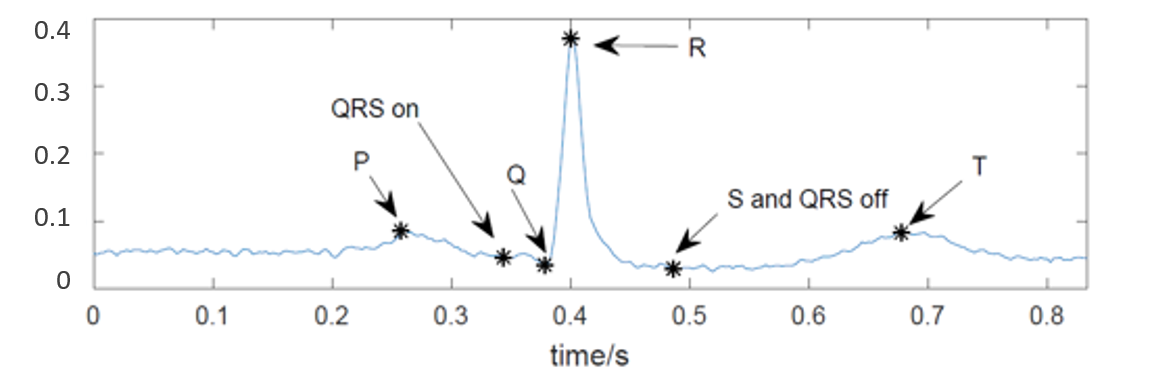
\includegraphics[scale=0.7]{Fig/fiducial_peaks2.png}  
 	\caption{Fiducial peaks within one cardiac cycle.}
 	\label{fig:fiducial_peaks}
 \end{figure}
 
The QRS complex is the most prominent wave and it contains the majority of the information of a ECG signal; therefore, most of the ECG delineation methods detect QRS complex prior to the detection of other peaks. Afonso \textit{et al.} proposed a method using filter banks to detect QRS complexes\cite{afonso1999ecg}. In this method, the signal is decomposed to several frequency bands. Fiducial peaks are thus detected using its morphological features in the decomposed signals. Sadhukhan \textit{et al.} proposed a method of detecting R peak by \textcolor{black}{thresholding the double difference signal of ECG data and comparing the relative amplitude within QRS region\cite{sadhukhan2012r}}. The performance of this method is validated using clinical ECG signals and has been proven to be promising. Some advanced machine learning techniques are also deployed to detect QRS complexes. In \cite{mehta2008svm}, \textit{Support Vector Machine} (SVM) is used to train a predictive model for QRS complex detection and achived 99.93\% accuracy. Other pattern recognition methods such as \textit{Hidden Markov Models} (HMM) are investigated and proved to be effecient in modeling and detecting characteritic peaks in ECG signals\cite{andreao2006ecg}. Wavelet decomposition is also frequently adopted for signal delineation due to the morphological similarity between wavelet basis functions and QRS complexes. As the QRS complex power spectrum is centered at the range of 5 to 30 Hz, the wavelet coefficients of the corresponding scale levels are frequently used for delineation purpose. In \cite{martinez2004wavelet}, QRS complexes are detected by thresholding wavelet coefficients at scales 1 to 4, then onset, offset and individual waves within QRS complexes are detected using the morphological characters of coefficient at scale 2. T and P waves are detected at scale 3 with a similar method approach. In the literature, some improvements have been proposed to eliminate false detection of R peaks by adding a fixed searching window of 160ms\cite{banerjee2012delineation}. 

\subsection{Feature Extraction and Classification}

After localizing the fiducial peaks within a cardiac cycle, we proceed with the next step of extracting informative features of the signal, which collectively convey meaningful information about the signal properties. %the classification system needs to extract information in the signal so that the signal could be represented by a set of features. 
Since the objective of designing an automatic classification system is to precisely predict types of sample signals, feature selection is usually performed to obtain a better performance and reduce the computation cost\cite{lagerholm2000clustering, prasad2003classification, autofs, ceylan2009novel, osowski2004support}. 

As the most significant wave within a ECG signal, the information of QRS complexes are proved to be the most important features for ECG classification systems. Lagerholm \textit{et al.} decompose QRS complexes with a set of Hermite basis functions and the decomposition coefficient are deplyed as ECG features to train a Self-Organizing Map (SOM), which achieved an average error rate of 1.5\% for 16 ECG types\cite{lagerholm2000clustering}. Prasad \textit{et al.} used discrete wavelet transform (DWT) to extract RR intervals between the current beat and previous or next beats. The two RR-intervals serve as input for training a neural networks, which achieves the average accuracy of 96.77\% in classifying 13 different arrhythmia types. De Chazal \textit{et al.} proposed two set of features: morphology and heartbeat interval features. They used different combinations of these features combined with Linear Discriminant Analysis to classify ECG signal into five arrhythmia types and selected the optimal feature set according to classification performance\cite{autofs}. The result shows that the sensitivity of detecting two major arrhythmia types can be improved by feature selection. R. Ceylan \textit{et al.}included RR interval as the only ECG feature to train a fuzzy clustering neural network that achieved an average detection rate of 98.35\%\cite{ceylan2009novel} . Osowski \textit{et al.} proposed two set of features including \textit{Higher Order Statistics} (HOS) and Hermite characterization of QRS complex to classify ECG signals with Support Vector Machine. Their final average error rate is at 1.82\%\cite{osowski2004support}. %Lannoy \textit{et al.}

\subsection{Patient-Specific ECG Classification}

The main drawback of the majority of aforementioned methods mentioned in the last section is the lack of inter-patient model adjustment. In order to generalize the ECG classification system to clinical applications, several methods which are more robust to inter-patient signal variation are proposed to address this issue\cite{Hu_et_al,deChazal2006,llamedo2012automatic,bbnn,ince2009generic,Kiranyaz}.

Hu \textit{et al.} proposed a patient-specific Mixture of Experts (MOE) classifier by incorporating personalized annotations provided cardiologists in the local classifier \cite{Hu_et_al}. The methods achieves patient-adapting capacity but requires further input from human experts. This MOE approach achieved an accuracy of 94.0\% for distinguishing \textit{Ventricular} beats from the other non \textit{Ventricular} types. Following the design of MOE, de Chazal and B. Reilly proposed an improved patient-adapting classifier by reducing the requirement of manual annotations to as few as 10 beats for training adaptive local classifier\cite{deChazal2006}. And Llamedo et al. designed an automatic classification system, which uses experts' assistance, but does not fully depend on the experts and can work independently\cite{llamedo2012automatic}. By implementing a special block-based neural networks (BbNNs), Jiang et al. achieved accuracies of 98.1\% and 96.6\% in distinguishing \textit{Ventricular} ectopic beats and \textit{supraventricular} ectopic beats from other types\cite{bbnn}. In \cite{ince2009generic}, particle swarm optimization (PSO) is combined with a neural network to optimize the network structure using patient-specific training data. Based on 1-D convolutional neural networks (CNN), Kiranyaz et al. proposed a flexible algorithm, which adjusts its parameters using information extracted from individual signals\cite{Kiranyaz}. The classifier demonstrates consistent performance over different ECG records achieving an accuracy between 98\% and 99\% for distinguishing VEBs from non-VEBs. (Acc = 98.9\%  Sen = 95.9\% Spe =  99.4\%). While this approach outperforms the aforementioned classification algorithms as it does not require expert further annotations, its performance reduces for some rare abnormal classes. 
 
\section{Contributions}

A crucial drawback of these patient-specific classification systems, recently proposed in the literature, is their failure in predicting abnormalities in advance. \textcolor{black}{These methods aim at improving classification performance by comparing generated labels with a ground truth for each beat and ignore the relationship between the generated labels and upcoming abnormalities. }%Conventionally, classifiers associate each sample with a label and optimize performance according to the uniformity of proposed label and ground truth. 
While in many common applications this approach generates satisfying results, it does not meet the needs of SCD prediction. %Combining patient-specific classifier and the character of ECG signal analysis, we proposed a patient-adaptable classification framework with a nonlinear transformation module to assist quantifying latent status between normal and abnormal types.

%In order to overcome this unpredictability, systems with advanced warning or predicting capacity are proposed in some recent researches. In \cite{advancewarning}, Kiranyaz et al. proposed an abnormal beat synthesis (ABS) approach to map normal beats to potential abnormal beats and thus generate analysis results in advance. The goal of normal-to-abnormal mapping is to model potential causes for spontaneous cardiac diseases. %The performance of warning on three consecutive abnormal beats are discussed, showing a promising 99.4% accuracy.

One of the main objectives of this work is to address the problem of forecasting by proposing the concept of \textit{yellow} and \textit{red alarms} and proving the fact that \textit{yellow alarms} can be indicators of upcoming \textit{red alarms}. \textit{Yellow alarms} are defined through a novel deviation analysis which assesses  the tendency of deviant normal alarms to one of the \textit{red alarm}. In order to realize such a deviation analysis, symmetry of different abnormality classes in feature space is desired. We propose a novel controlled nonlinear transformation that maps the original feature space into a new space that presents the desired symmetry. %two different feature space transformations to optimize the predicting capacity of personalized classifier for applications using biomedical signals. 
To elaborate more on the symmetry of abnormal classes in the feature space, we assume that there are one normal class and multiple abnormal classes for a signal while latent states exists for some of the normal samples that represent slight deviations towards abnormalities. %normalities with deviation towards abnormalities, indicating information regarding subsequent abnormalities. 
By distinguishing  latent states, the designed automated system is capable to generating a \textit{yellow alarm} which indicates a high probability of the presence of some upcoming abnormalities (\textit{red alarms}) of the same type. Therefore, the contribution of this work can be summarized as:

\begin{itemize}
    \item Propose a novel self-configuring patient-adaptive framework which incorporates a personal classifier into the predictive modeling;
    \item Utilize a kernel-based method as a spatial transformation with parameters optimized using multi-objective particle swarm optimization (MOPSO) for the purpose of deviation quantification;
    \item Design a controlled spatial transformation with deterministic mapping function to optimize cluster topology for predictive analysis
    \item Propose a deviation quantification method based on cosine similarities, which is capable of generating \textit{red alarms} for upcoming abnormalities
\end{itemize}


\section{Organization of Thesis}

In the following chapters, details of the proposed classification framework are presented after reviewing the introductory concepts and related works. Chapter 2 provides a general information about the utilized ECG dataset and the general framework used in proposed classification system. Chapter 3 describes the details of nonlinear transformation with kernel methods and presents the experimental results using kernel transformation. With the concept of nonlinear transformation, chapter 4 introduces an optimized spatial transformation with a novel deterministic mapping function. The experimental result for the spatial transformation method is presented section \ref{sec:result_spatial}. Finally, the experimental results for the proposed methods in chapter 3 and chapter 4 are studied and compared. More importantly, the predicting capacity of the proposed system is studied and analyzed in this chapter. Based on the experimental results, we introduce some potential directions to further improve the system in terms of classification and predicting accuracy.
